% -----------------------------------------------
% Template for ISMIR Papers
% 2017 version, based on previous ISMIR templates

% Requirements :
% * 6+n page length maximum
% * 4MB maximum file size
% * Copyright note must appear in the bottom left corner of first page
% * Clearer statement about citing own work in anonymized submission
% (see conference website for additional details)
% -----------------------------------------------

\documentclass{article}
\usepackage{ismir,amsmath,url}
\usepackage[nocompress]{cite}
\usepackage{graphicx}
\usepackage{color}
\usepackage{array}
\usepackage{tabularx}
\usepackage{arydshln}

\newcommand{\carl}[1]{\textcolor{blue}{#1}}
\newcommand{\izzy}[1]{\textcolor{red}{#1}}
\newcommand{\maciek}[1]{\textcolor{green}{#1}}
\newcommand{\jason}[1]{\textcolor{orange}{#1}}




%\renewcommand\note[1]{}


%\newcommand\myworries[1]{\textcolor{red}{#1}}
% Title.
% ------
%\title{Paper Template For ISMIR \conferenceyear}
\title{PLAYER IDENTIFICATION FOR TRADITIONAL IRISH FLUTE RECORDINGS}

% Note: Please do NOT use \thanks or a \footnote in any of the author markup

% Single address
% To use with only one author or several with the same address

%\oneauthor
%{Islah Ali-MacLachlan, Maciej Tomczak, Carl Southall, Jason Hockman}
%{DMT Lab, Birmingham City University \\ {\tt islah.ali-maclachlan, maciej.tomczak, carl.southall, jason.hockman} \\{\tt @bcu.ac.uk}}

% Three addresses
% --------------
\threeauthors
  {First Author} {Affiliation1 \\ {\tt author1@ismir.edu}}
  {Second Author} {\bf Retain these fake authors in\\\bf submission to preserve the formatting}
  {Third Author} {Affiliation3 \\ {\tt author3@ismir.edu}}
% ---------------


\sloppy % please retain sloppy command for improved formatting

\begin{document}

%
\maketitle
%
\begin{abstract}

The abstract should be placed at the top left column and should contain about 150-200 words.

Irish Traditional Music (ITM) has progressed from its roots of social dance music to become a medium for listening. Represented at several large-scale music festivals in Europe and the US, and over 1500 weekly 'sessions' where musicians can meet and share repertoire, the indigenous music of Ireland has a large, international audience \cite{vallely_companion_2011}. 

Playing of the wooden simple system flute  in ITM was historically linked predominantly to the west and northwest of Ireland. The Irish cultural revival has allowed the flute to play a wider role as an intrinsic part of the sound of ITM alongside tin whistles, accordions, and fiddles \cite{williams_irish_2010}. 



 Traditional flute players are individuated based on their use of techniques such as ornamentation, phrasing and articulation 
\cite{mccullough_style_1977,hast_music_2004, keegan_parameters_2010, larsen_essential_2003} alongside idiosyncratic timbral differences \cite{ali-maclachlan_quantifying_2013, widholm_silver_2001, ali-maclachlan_towards_2015}. Mastery is judged by creativity and technical ability within the stylistic bounds of traditional music and distinctive characteristics often develop organically as a player learns and refines their skills.  

In order to determine stylistic differences between players, we must first develop methods to detect these differences in audio signals. We evaluate recordings produced by six accomplished traditional flute players, all playing music from a predetermined corpus offering a range of typical modes and rhythms.


\end{abstract}
%
\section{Introduction}\label{sec:introduction}


\sloppypar{Irish Traditional Music (ITM) has progressed from its roots of social dance music to become a medium for listening. Represented at several large-scale music festivals in Europe and the US, and over 1500 weekly 'sessions' where musicians can meet and share repertoire, the indigenous music of Ireland has a large, international audience \cite{vallely_companion_2011}. 

Playing of the wooden simple system flute  in ITM was historically linked predominantly to the west and northwest of Ireland. The Irish cultural revival has allowed the flute to play a wider role as an intrinsic part of the sound of ITM alongside tin whistles, accordions, and fiddles \cite{williams_irish_2010}. 

%\begin{figure}[h]
%\begin{center}
%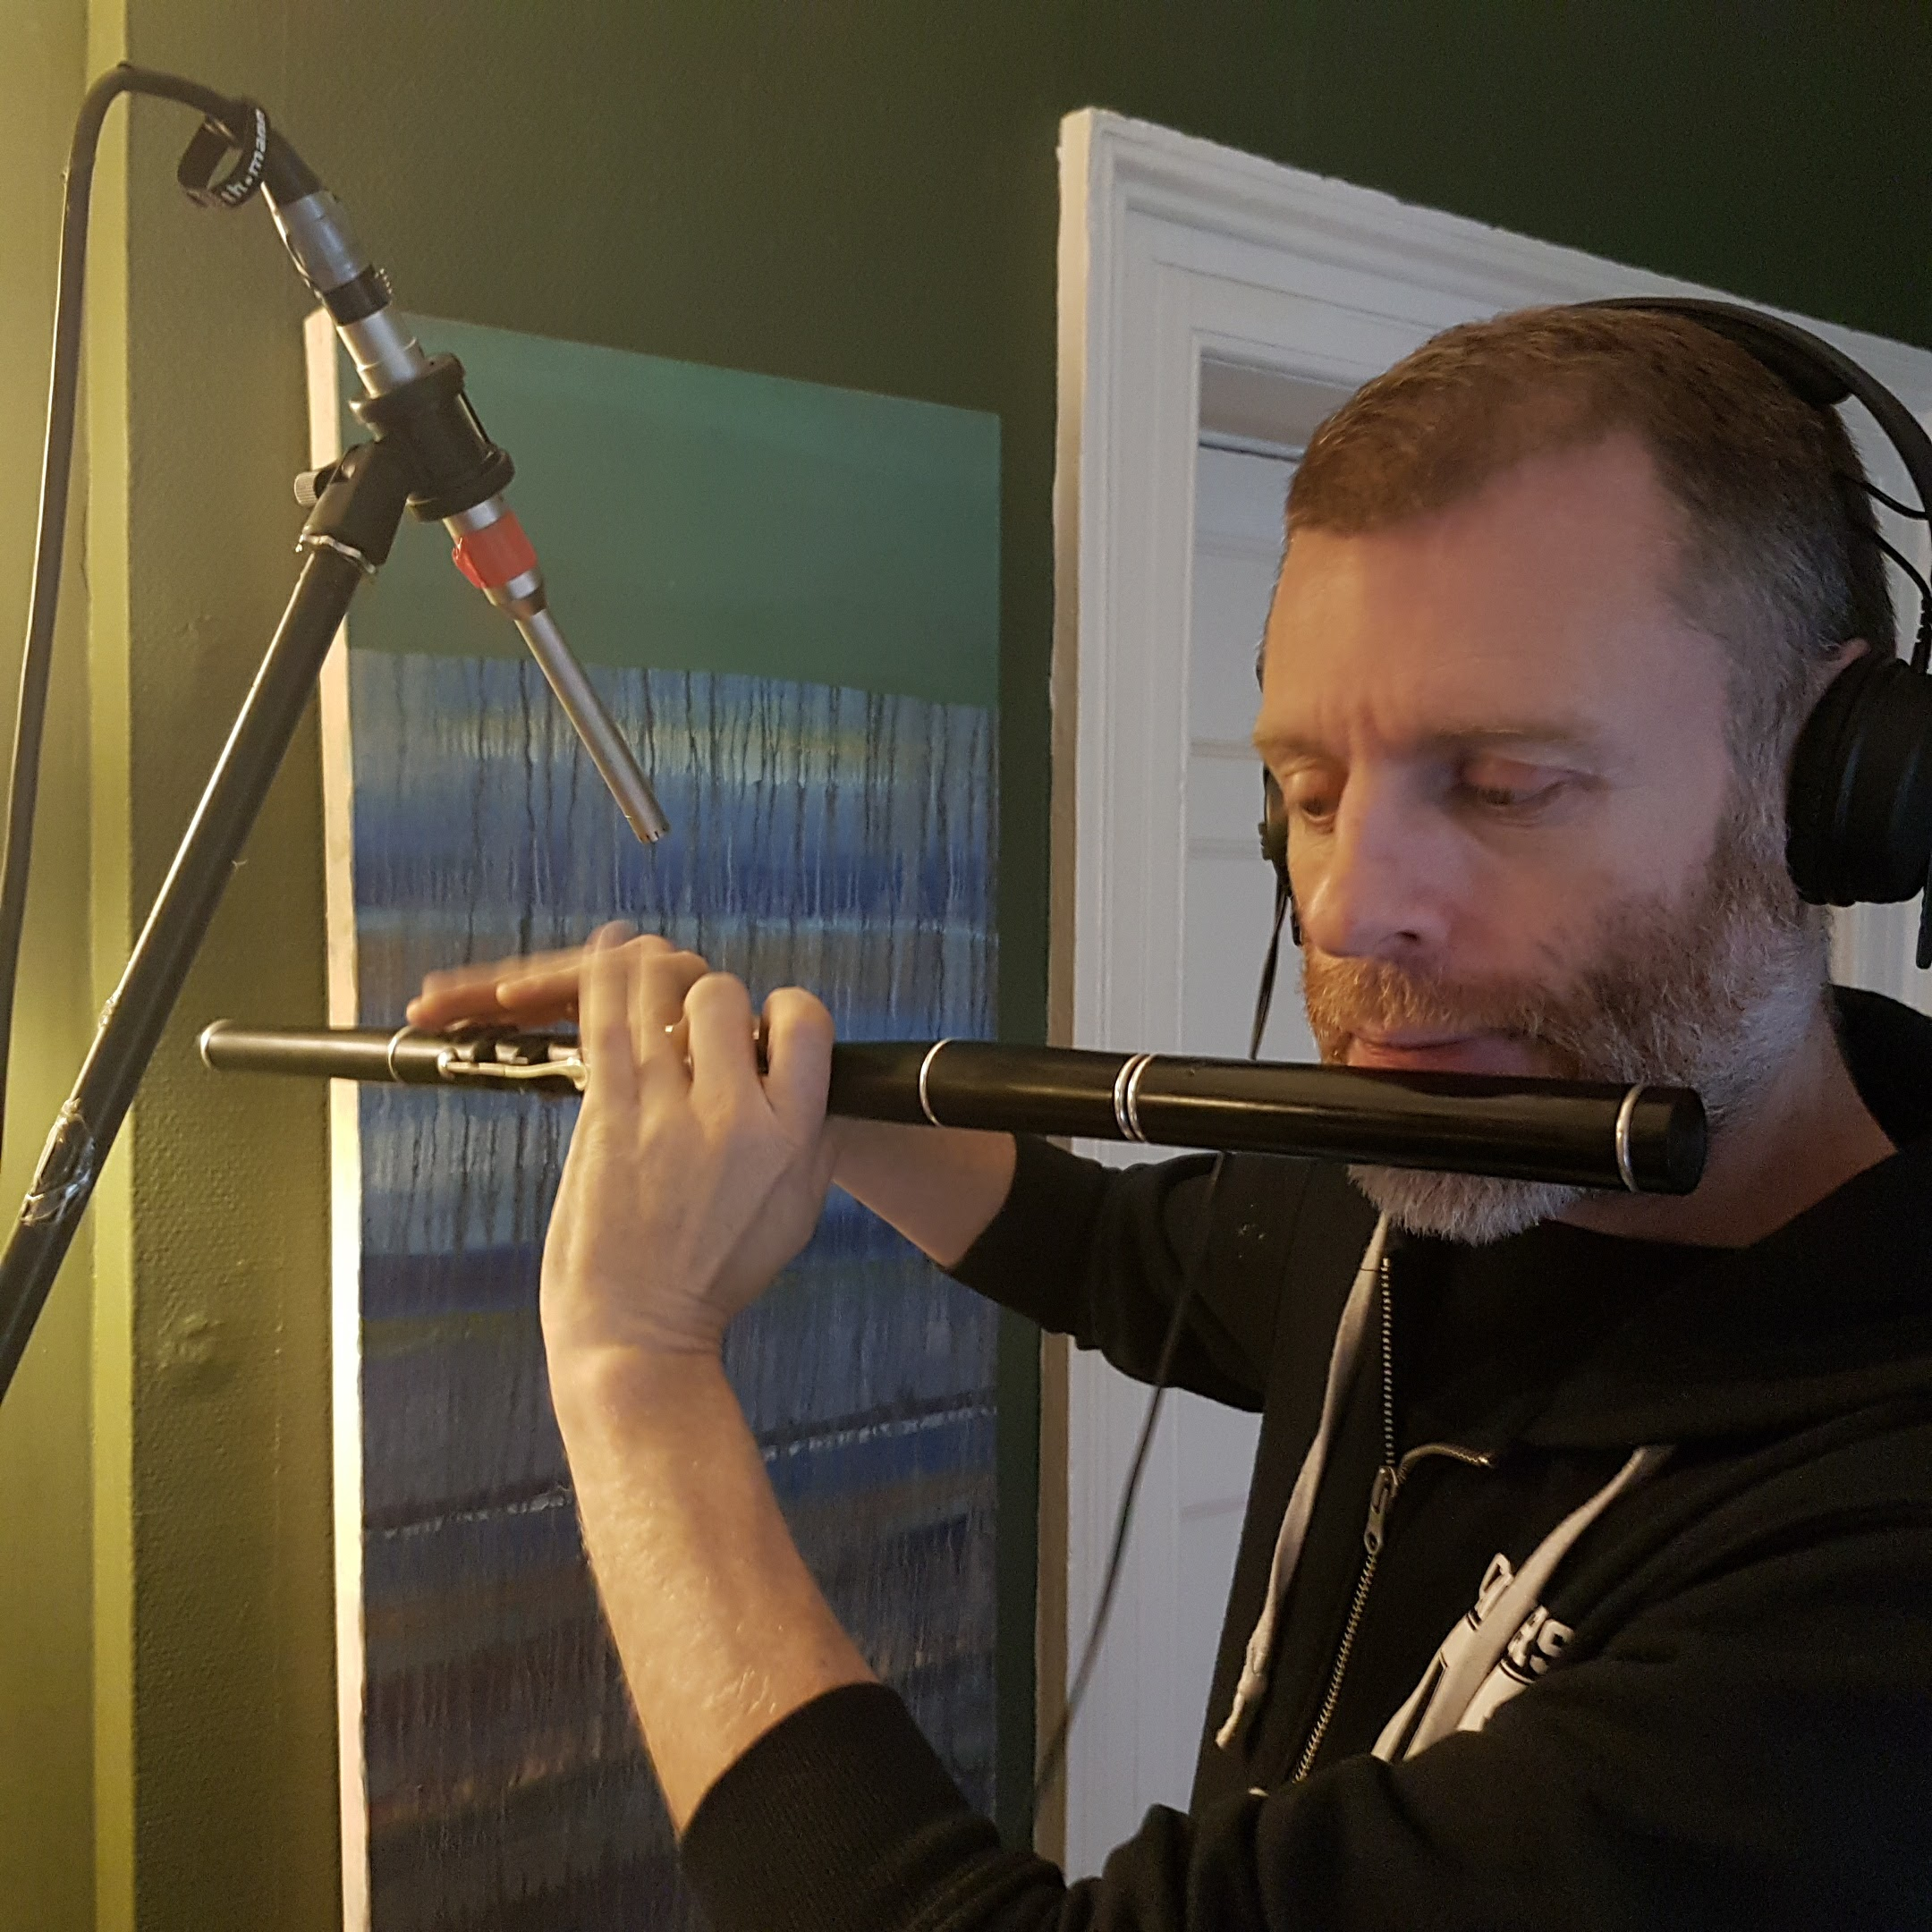
\includegraphics[width=0.45\textwidth]{figs/p4-1.jpg}
%\caption{Player with keyed blackwood simple system flute.}
%\label{fig:flute1}
%\end{center}
%\end{figure}

 Traditional flute players are individuated based on their use of techniques such as ornamentation, phrasing and articulation 
\cite{mccullough_style_1977,hast_music_2004, keegan_parameters_2010, larsen_essential_2003} alongside idiosyncratic timbral differences \cite{ali-maclachlan_quantifying_2013, widholm_silver_2001, ali-maclachlan_towards_2015}. Mastery is judged by creativity and technical ability within the stylistic bounds of traditional music and distinctive characteristics often develop organically as a player learns and refines their skills.  

In order to determine stylistic differences between players, we must first develop methods to detect these differences in audio signals. We evaluate recordings produced by six accomplished traditional flute players, all playing music from a predetermined corpus offering a range of typical modes and rhythms.

\subsection{Related work} \label{sec: Related Work}

The influence of instrument and player in the production of flute timbre has been studied by changing the flute material and wall thickness, showing that each has little effect on the overall sound produced and that individual players contribute more to spectral differences \cite{backus_effect_1964, coltman_effect_1971, widholm_silver_2001}. Analysis of three players across six wooden simple system flutes showed significant differences between long-term average spectrum plots of different players when compared to a single musician playing different flutes. Analysis of short-term harmonic magnitudes was also performed using the stable central portion of each note, showing differences between magnitudes of the first four harmonics \cite{ali-maclachlan_quantifying_2013}. A dataset of 20 commercial recordings containing four traditional Irish solo flute melodies from each of five players was analysed by comparing harmonic magnitudes of all instances of particular notes, with variable results \cite{ali-maclachlan_towards_2015}. %Results varied between 18.8\% and 67.7\% accuracy 

The methods above rely on signal processing but state of the art identification techniques use probabilistic modelling. Convolutional neural networks (CNN) have been used successfully with input features derived from spectrograms \cite{lee_unsupervised_2009} and Mel-frequency cepstral coefficients (MFCC) representing timbre, tempo and key variations \cite{li_automatic_2010}. A CNN was trained to perform artist and genre recognition on the 'Million Song Dataset' \cite{bertin-mahieux_million_2011} using segments related to note onsets and feature vectors containing timbre and chroma components \cite{dieleman_audio-based_2011}. Lidy \& Schindler \cite{lidy_parallel_2016} used CNN to classify genre, mood and composer and achieved the highest results in MIREX 2016 using a 40-band Mel filter.

Costa et al \cite{costa_evaluation_2017} reinforced the effectiveness of CNN for music genre classification, performing analysis against support vector machines on three separate databases containing Western, Latin and African music. The CNN system compared favourably in a number of scenarios, particularly in the case of African music where the sources were largely field recordings. This method showed favourable results with multiple class types labelled country, function, ethnic group and instrumentation. Individual instrument classification is discussed in \cite{park_musical_2015} and as part of an ensemble in \cite{han_deep_2017}.

Motivation


The remainder of this paper is structured as follows: Section \ref{sec:method}  details the method of segmentation, feature extraction and classification. In Section \ref{sec:evaluation} we discuss evaluation of.... Results of the studies into ... are presented in Section \ref{sec:results} and finally conclusions and further work are discussed in Section \ref{sec:conclusions}.

\begin{figure*}[t]
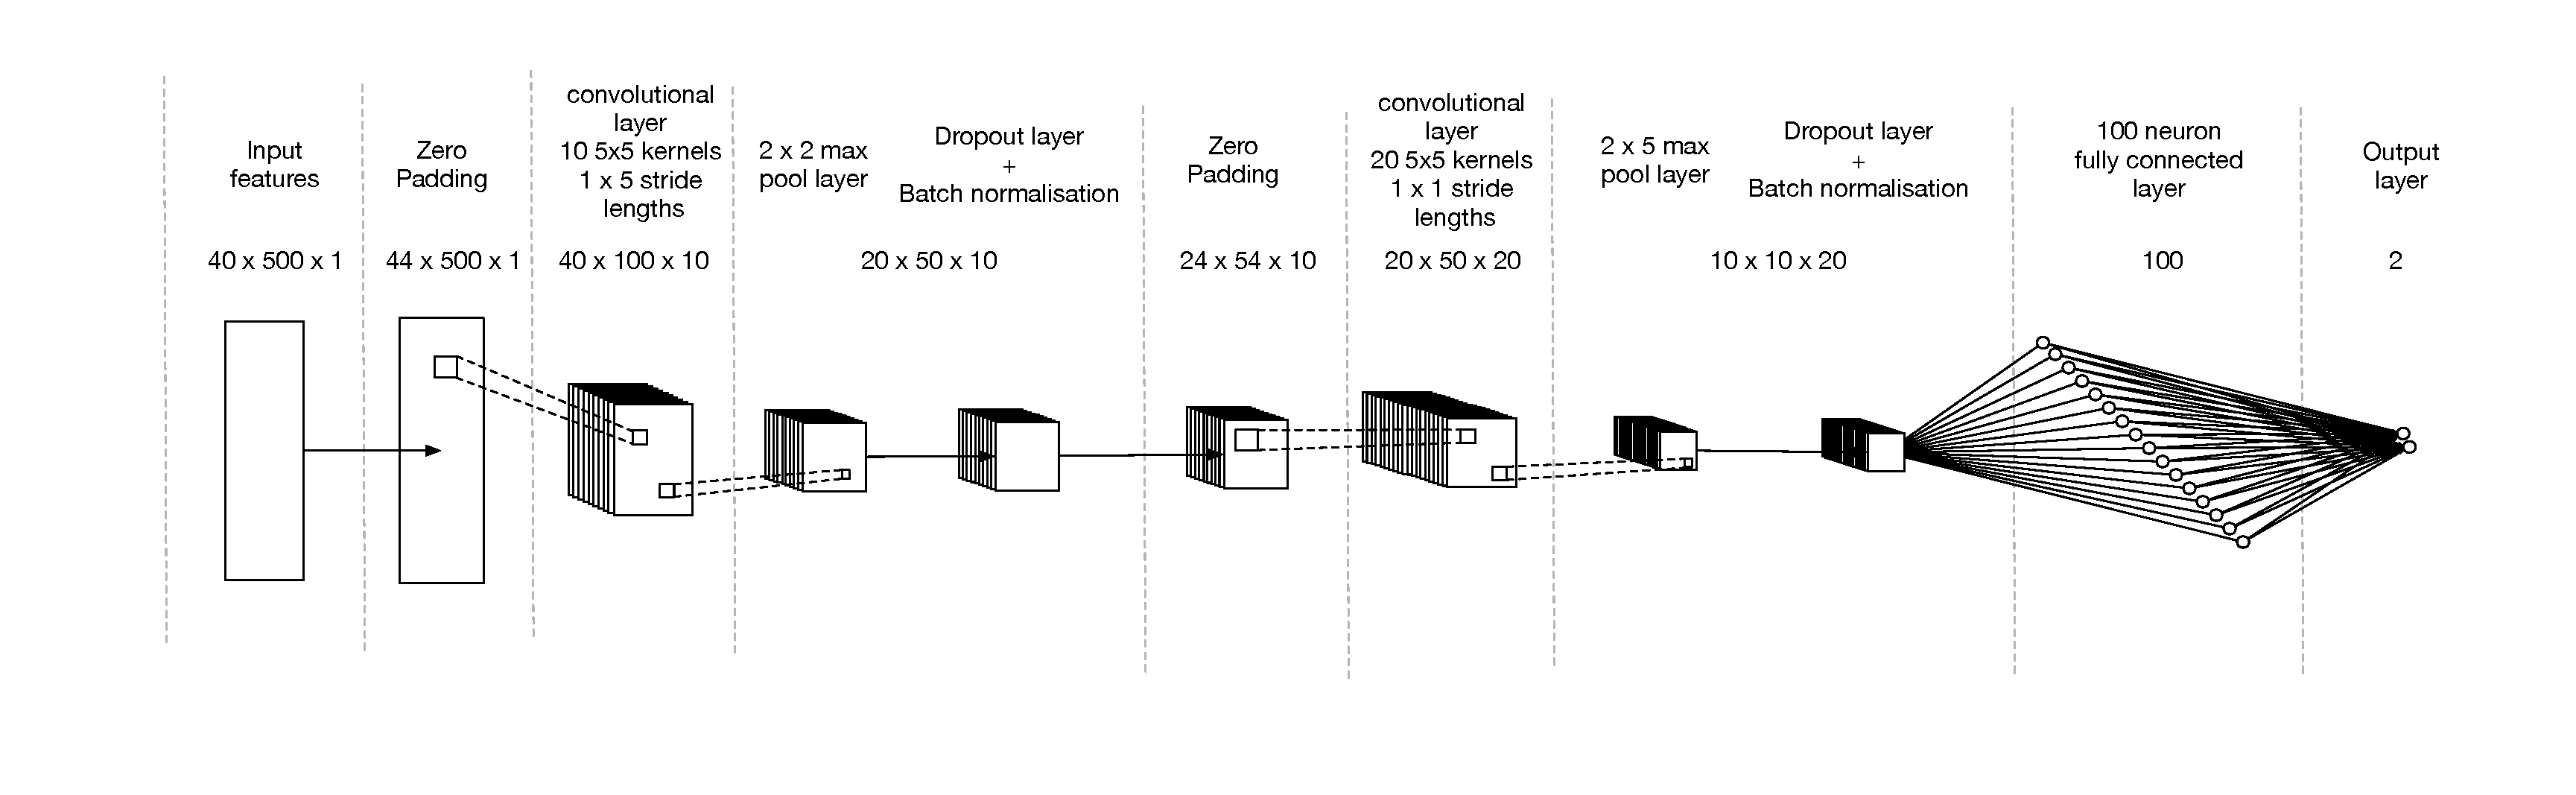
\includegraphics[width=1\textwidth]{figs/CNNDiagramPD}
\caption{Overview of the proposed implemented CNN system.}
\label{CNNDiagram}
\end{figure*}

\section{Method} \label{sec:method}

Introductory paragraph

%MFCC extraction implemented using http://www.ee.columbia.edu/~dpwe/resources/matlab/rastamat/mfccs.html

%Figure \ref{fig:SignalFlow} shows an overview of the proposed method. We extract features from audio segments representing events (notes, cuts, strikes) and propose an event type classification approach using the segmented event features. 
%
%For a fully automated method we use onset detection for segmentation. Event features are then extracted from inter-onset intervals (IOI). These features are used in a supervised learning algorithm to classify the segments as one of three distinct classes: notes, cuts and strikes. For onset detection, we attempt to use the top-performing algorithm from the evaluation presented in Section \ref{sec:Onset Detection Evaluation}, and in the following discuss only the remaining feature extraction and classification stages.
%
%\begin{figure}[h]
%\begin{center}
%
%\vspace{6mm}
%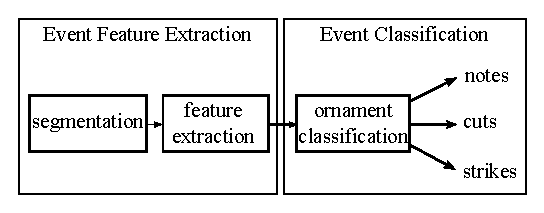
\includegraphics[width=0.45\textwidth]{SignalFlow.eps}
%
%\caption{Overview of the proposed classification method of notes, cuts and strikes in flute signals. The first phase shows feature extraction from segmented audio events and the second phase shows classification of the events.}
%\label{fig:SignalFlow}
%\end{center}
%\end{figure}



\subsection{Convolutional neural networks (CNN)}
In order to capture the stylistic differences between each player we divide recordings into 5 second segments. We then extract timbral features as these are important in class distinction. Each player contributes distinct timbral features as part of their style. For that purpose we extract 40 MFCCs, excluding the first coefficient, to accommodate for differences in timbre over a range of played notes.%

%
CNNs enable larger input feature sizes to be used by first reducing the dimensionality of the features using a shared weighted kernel and pooling before they are input into a fully connected layer. This ability has enabled CNNs to achieve higher accuracies than recurrent neural networks in closed related fields including onset detection, beat detection and downbeat detection. REFEERENCES  An overview of the implemented CNN ADT systems with different input feature sizes is outlined in Figure... REF. All of the implement versions consist of two sets of convolutional, max pooling, dropout, and batch normalisation layers before a 100 neuron fully connected layer and a two neuron softmax output layer. The output $h$ of a two-dimensional convolutional layer with a rectified linear unit transfer function is calculated using:

\begin{equation}\label{eqn:conv}
 h^f_{ij}=r\Bigg(\sum_{l=0}^{L-1}\sum_{m=0}^{M-1} W^f_{ml}x_{(iu+l)(jv+m)}+b^f\Bigg)
\end{equation}

where $x$ is the input features, $W$ and $b$ are the shared weights and bias and $f$ is the feature map. $L$ and $M$ are the dimensions of the shared weight matrix and $I$ and $J$ are the output dimensions of that layer. $u$ and $v$ are the stride lengths and the equation for the rectifier linear unit transfer function $r$ is:

\begin{equation}\label{eqn:rect}
r(\phi)=max(0,\phi)
\end{equation}

Before the features $x$ are input into the network they are zero padded.

The output of the convolutional layer $h$ is then processed using a max pooling layer where the maximum of $a$ by $b$ sub-regions is taken. Dropouts are then performed on the output of the max pooling layer with a dropout probability of 0.25 and batch normalisation is implemented. \carl{IN DEPTH DETAIL ON BATCH NORM!}.

The output of the second batch normalisation $h_{bnL}$ layer is then input into a dense fully-connected layer ($Q=h_{bnL}$) Equation.{\ref{eqn:output} with a rectifier linear unit transfer function ($\sigma(\phi)=r(\phi)$) Equation.\ref{eqn:rect}. The output layer of the implemented CNNs is the same as the output layer of the SABRNN systems with the input to the layer being the output of the fully connected layer ($Q=h_fc$).


\subsection{Implementation}

The Tensorflow Python library is used to implemented our proposed system. 

\subsubsection{Input Features}

%To extract features from the audio segments the input audio (mono WAV files) is down sampled to 11,025 Hz. Following the approach in \citet{mauch2010simultaneous} we calculate the MFCC and chroma features using a Hanning window of 1024 samples with 50\% overlap. The extracted features are then normalised to the range [0,1] for every corresponding feature type. Each audio segment is assigned to its class $\Omega$ (e.g. note). An $n$ x $26$ matrix $F_\Omega$ is created, where $n$ represents the number of segments with 26 features (i.e., MFCCs, chroma, durations).
%
%Each $F_\Omega$ segment appears in the context of musical patterns such as rolls, shakes or just consecutive notes in the recording. To account for the rhythmic, timbral and pitch changes of each event type in the context of these patterns, we concatenate the first derivatives of all features into every $F_\Omega$ segment.
%Audio segments are then classified into note, cut and strike classes using a feed-forward neural network.

\subsubsection{Training Procedure}

The implemented models are trained using the Adam optimizer and a learning rate of 0.003.  Mini-batch gradient descent is used with batch sizes of 250. Training is stopped when a minimum of 50 iterations have commenced and the
validation set accuracy has not increased between iterations. The weights are initialized using a scaled uniform distribution \cite{DBLP:journals/corr/Sussillo14}
and biases are initialized to 0. Cross entropy is used as the loss function.

%\begin{figure}[h]
%\begin{center}
%
%\vspace{6mm}
%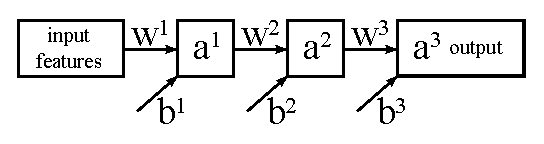
\includegraphics[width=0.45\textwidth]{NeuralNetworkArchitecture.eps}
%\caption{Neural network architecture containing two hidden layers $a^1$ and $a^2$, with weights $w$ and biases $b$.}
%\label{fig:NeuralNetworkArchitecture}
%
%\end{center}
%\end{figure}
%
%The proposed neural network, shown in Figure \ref{fig:NeuralNetworkArchitecture}, consists of two hidden layers containing 20 neurons each. Back propagation is used to train the neural network, updating the weights and biases iteratively using scaled conjugate gradient of the output errors. A maximum iteration limit is set to 10,000 and the weights and biases are initialised with random non-zero values to ensure that training commenced correctly. A validation set is used to prevent over-fitting and cross entropy is used for the performance measure.
%
%The output for each layer of an $L$ layered neural network can be calculated using:
%\begin{equation}
%a^{(l)} = f_{l}( a^{(l-1)} W^{l}+b^{l}),
%\end{equation}
%where, $a^l$ is the output at layer $l$ and $W$ and $b$ are the weight and bias matrices. The transfer function is determined by the layer, as shown in Eq. \ref{eq:layerFn}.
%
%\begin{equation}\label{eq:layerFn}
%f_{l}(x)=\left\{
%\begin{array}{ll}
% 2/(1+e^{-2x})-1, & l\neq L\\
% y=e^x/(\sum e^x), & l=L.\\
%\end{array}
%\right.
%\end{equation}
% 
%\noindent Classification is performed by finding the index of the maximum value within the output from the neural network.
%
%\section{Evaluation}\label{sec:evaluation}
%As the performance of the proposed method depends heavily on the accuracy of the chosen onset detection method, the aim of our first evaluation is to determine the best performing onset detection algorithm. We then perform an evaluation of our note and ornament classification.

\section{Evaluation} \label{sec:evaluation}

\subsection{Dataset}\label{sec:dataset}
For these evaluations, we require a dataset that is representative of a range of respected players with individual stylistic traits. The dataset comprises of 247 recordings of traditional 'tunes' played on solo flute and includes 168 recordings of 6 experienced players alongside 79 released recordings of 9 professional players detailed in \cite{ali-maclachlan_islah_note_2016}. 

The dataset is representative of the four most popular melodic styles, namely the reel, jig, hornpipe and polka \cite{hast_music_2004}. The structure of most traditional melodies in ITM can be attributed to two scales, D and G, and four classes defined by the ending note of the tune and given the solfa name Doh, Ray, Soh and Lah \cite{breathnach_folk_1996, o_canainn_traditional_1978}. 

The corpus of tunes shown in Table {\ref{tab:corpusTunes} was chosen to be representative of a typical player repertoire and to represent a range of scales and classes. 6 players played each tune twice without tempo restriction and twice in time with a click track played through headphones and set to represent a typical speed according to \cite{breathnach_ceol_1963}. Players also recorded two other tunes picked from their own repertoire.

\begin{table}[]
\centering

\label{tab:corpusTunes}
\begin{tabular}{|l|c|c|c|}
\hline
\multicolumn{1}{|c|}{\textbf{Tune Title}} & \textbf{Type} & \textbf{Scale} & \textbf{\begin{tabular}[c]{@{}c@{}}Ends\\ on\end{tabular}} \\ \hline
Maids of Mount Cisco                      & Reel          & G              & Ray                                                         \\ \hline
The Banshee                               & Reel          & G              & Soh                                                         \\ \hline
Cooley's Reel                             & Reel          & G              & Lah                                                         \\ \hline
Banish Misfortune                         & Jig           & G              & Doh                                                         \\ \hline
Morrison's Jig                            & Jig           & D              & Ray                                                         \\ \hline
The Home Ruler                            & Hornpipe      & D              & Doh                                                         \\ \hline
\end{tabular}
\caption{Corpus recorded by all players detailing tune type, scale and ending note}
\end{table}


\subsubsection{Recording} \label{sec:recording}
The recordings were collected as 16-bit/44.1kHz WAV files using a Thomann MM-1 measurement microphone connected to an Audient ID14 audio interface. The microphone was positioned above the middle of the flute in order to minimise wind noise. 
 



\subsection{Evaluation of methods}\label{sec:evalmeth}



%The dataset represents a wide range of musicians and playing styles, although two main approaches can be observed with some players choosing either to play rhythmically using mainly breath control or rely more on finger ornaments such as cuts, strikes and rolls \citep{kokuer_towards_2014}.

%A corpus of 79 solo flute recordings, consisting of includes 41 reels, 22 jigs, 10 polkas and 6 hornpipes,  was assembled to allow analysis of stylistic features. 
%A corpus of 99 traditional flute recordings were manually annotated in order to create a digital library for stylistic analysis. From the full corpus, we omitted the twenty tunes recorded by Larsen as they are sourced from the CDs accompanying \citet{larsen_essential_2003}. Some of the recordings are training exercises and therefore not representative of typical playing. A number of these tunes are used in the datasets for \citet{kelleher_onset_2005-1} and \citet{kokuer_automated_2014}.
%The above paragraph exists because the Gainza (and Kokuer) analyses used the Larsen dataset but I feel it is not representative of "real" playing.

\subsection{Onset detection evaluation}
\label{sec:Onset Detection Evaluation}

% Detecting onsets is an important step in automatically finding individual notes and ornaments, both of which are important components in defining player style \citep{keegan_parameters_2010}.
%In this evaluation we measured how well eleven onset detection algorithms were capable of identifying onsets related to notes, cuts and strikes within real-life flute recordings. We reviewed the wind instrument class results from MIREX and examined various studies that concerned detection of soft onsets within these instruments. 
%
%Specialised methods for soft onset detection have been proposed in the literature. \emph{SuperFlux} by \citet{bock_maximum_2013-2} calculates the difference between two near short-time spectral magnitudes and is optimised for music signals with soft onsets and vibrato effect in string instruments. \emph{ComplexFlux} by \citet{bock_local_2013-1} is based on the \emph{SuperFlux} algorithm with the addition of a local group delay measure that makes this method more robust against loudness variations of steady tones. Similarly, \emph{LogFiltSpecFlux} introduced in \citet{bock_evaluating_2012-3} was designed to deal with onsets of various volume levels but was optimised for real-time scenarios. 
%
%In addition, there are several other onset detection methods proposed in the literature that we tested. The \emph{OnsetDetector} by \citet{eyben_universal_2010} processes the input signal both in the forward and backward manner and outputs peaks that represent the probability of an onset at the detected position. The \emph{Energy} \citep{masri_computer_1996}, \emph{Spectral Difference} \citep{foote_beat_2001}, \emph{Spectral Flux} \citep{dixon_onset_2006-1} and \emph{Kullback-Leibler} (KL) \citep{hainsworth_onset_2003} represent detection functions solely based in the spectral domain. \citet{brossier_automatic_2006} presented a modification to the KL algorithm shown as \emph{Modified Kullback-Leibler} in our evaluation. The  \emph{Phase-based} method by \citet{bello_phase-based_2003} looks at phase deviation irregularities in the phase spectrum of the signal. Lastly, the \emph{Complex Domain} approach by \citet{duxbury_complex_2003} combines both the energy and phase information for the production of a complex domain onset detection function. Peak-picking for the evaluate approaches is performed with $Madmom$\footnote{https://github.com/CPJKU/madmom} and $Aubio$\footnote{http://aubio.org/} MIR toolboxes.
%
%The onset detection results were calculated using the standard precision, recall and F-measure scores that measure performance of each onset detection algorithm. Precision and recall are determined from the detected flute onsets if reported within 25 ms on either side of the ground truth onset times. The mean F-measure is calculated by averaging F-measures across recordings.


\subsection{Note and ornament classification evaluation}

%To assess the performance of our presented note and ornament classification method, we perform two evaluations using the dataset from Section \ref{sec:dataset}. In the first evaluation, we attempt to determine the worth of the chosen classification method and selected features alone. In this experiment, we rely on the manually annotated note onsets to segment the audio prior to the feature extraction and classification stages. In the second evaluation, we seek to determine the viability of a fully automated ornament detection approach that relies on onset detection for segmentation. In this evaluation we employ the top performing onset detection algorithm found in the onset detection evaluation detailed in Section \ref{sec:Onset Detection Evaluation}. For the training of the automated method only the true positive onsets will be used to ensure that the neural network is trained with the features corresponding to their correct classes. 
%
%To ensure an approximately equal proportion of training examples per class, we reduced the number of notes per recording to 6\%, cuts to 30\% and left in all strikes due to the proportion of these classes in the dataset. The classification evaluation is then performed using 5-fold cross validation.


\section{Results}\label{sec:results}

\subsection{Sub1}



\subsection{Sub2}





\subsection{Sub3}






\section{Conclusions and Future Work} \label{sec:conclusions}
%In this paper we present a note, cut and strike detection method for traditional Irish flute recordings. Our chosen approach to this problem is that of inter-onset segment classification using feed-forward neural networks. To evaluate the effectiveness of this approach we first conducted an evaluation of various onset detection algorithms on our dataset with the hope of using this method as a first step in the feature extraction. 
%
%When using ground truth onset annotations, we achieved 86\%, 70\% and 74\% accuracies for note, cut and strike classification respectively. When using detected onsets to train the neural network we achieved poor classification results. We then performed an analysis of the detected onsets and the context in which they appear to establish both the degree of the errors and the musical patterns in which they occur.
%
%In the future we intend to work on improving the automated detection of note events. We will also develop note and ornament classification methods with additional features and other neural network architectures (e.g., recurrent neural networks, networks with long short-term memory) in order to capture trends that appear in time-series data. We also plan to investigate how well the proposed system generalises to other instruments that are characterised by soft onsets such as the tin whistle and fiddle.



%\section{Acknowledgements}









% For bibtex users:
\bibliography{ISMIR2017}

% For non bibtex users:
%\begin{thebibliography}{citations}
%
%\bibitem {Author:00}
%E. Author.
%``The Title of the Conference Paper,''
%{\it Proceedings of the International Symposium
%on Music Information Retrieval}, pp.~000--111, 2000.
%
%\bibitem{Someone:10}
%A. Someone, B. Someone, and C. Someone.
%``The Title of the Journal Paper,''
%{\it Journal of New Music Research},
%Vol.~A, No.~B, pp.~111--222, 2010.
%
%\bibitem{Someone:04} X. Someone and Y. Someone. {\it Title of the Book},
%    Editorial Acme, Porto, 2012.
%
%\end{thebibliography}

\end{document}
